(by Vipin Singh)

\p
In this chapter we will discuss the timeline of the project, for which we show a GANTT chart in figure \ref{fig:timeline_gantt} showing the roadmap for implementing the business idea.

\begin{figure}[H]
    \centering
    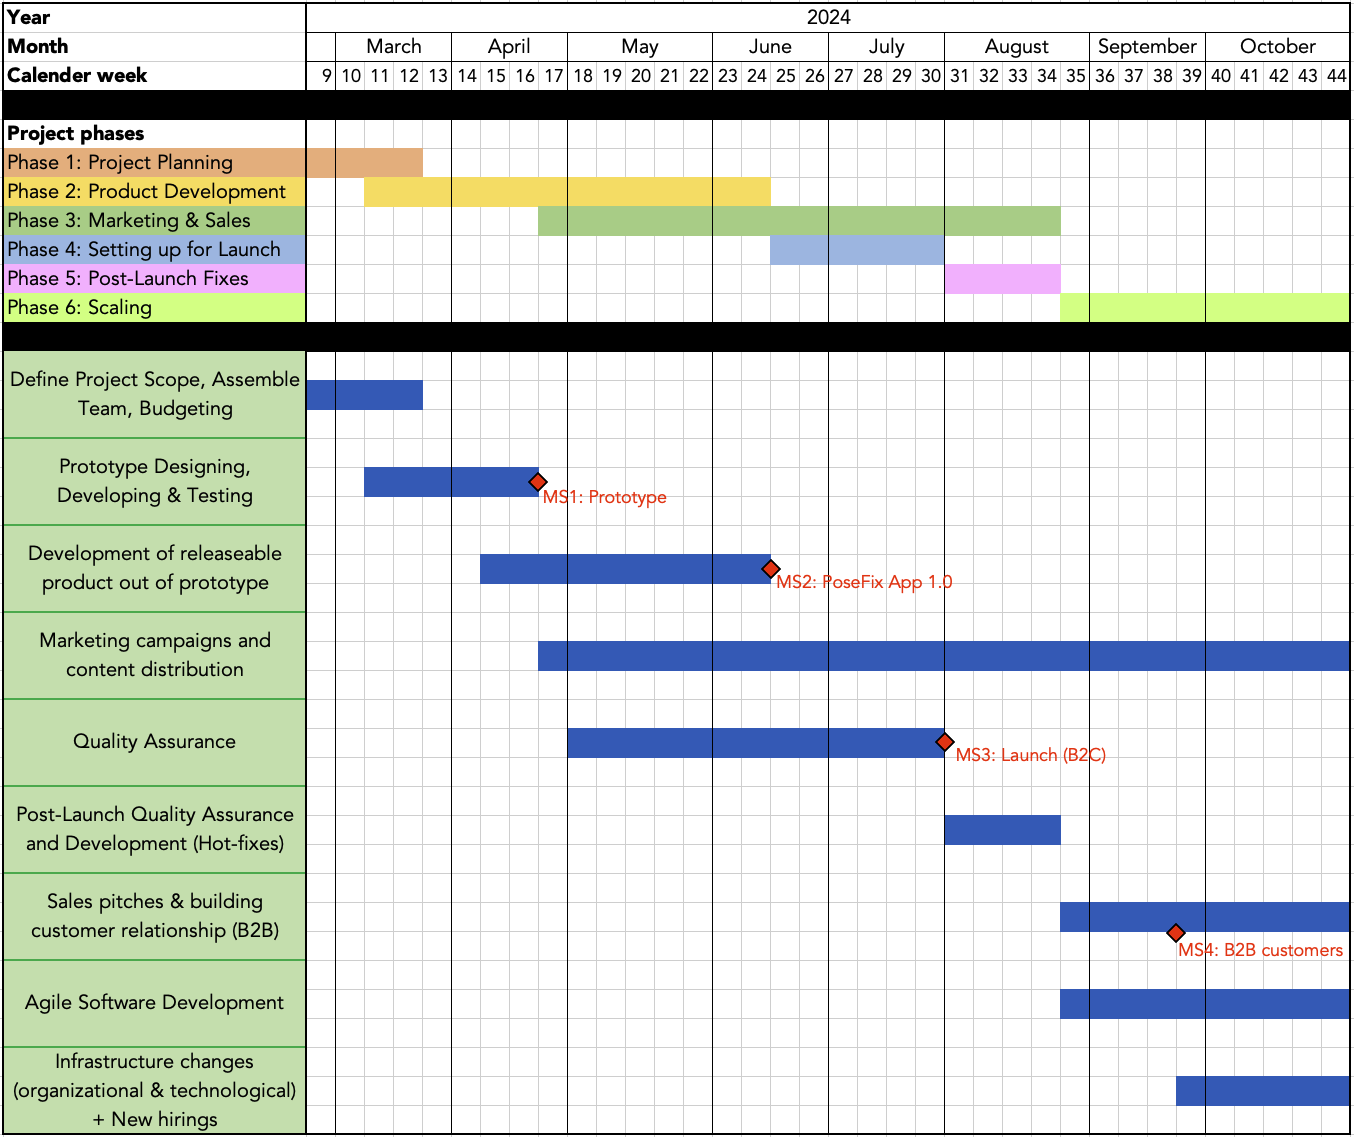
\includegraphics[width=\textwidth]{figures/GANTT_timeline.png}
    \caption{Timeline of the project as a GANTT chart}
    \label{fig:timeline_gantt}
\end{figure}

To have a clear structure of the project, we mapped the different task into six phases.
The first phase is the \textbf{Project Planning} phase.
This phase will be used to set up the project teams, define the scope of the project and already start with budgeting.
In total we planned to spend 4 weeks on this phase.
After 2 weeks though we might be already able to start with the next phase.

\p
The second phase is the \textbf{Product Development}.
This phase will start with designing the prototype.
The initial designs of the prototype can also therefore already be discussed in the project planning phase.
After the design has been agreed on, the Product Development team can start developing and testing the prototype.
In total we assume that this task will take 6 weeks.
The prototype is also our first milestone in this project.
As soon as the prototype is ready, the next phase can start, while the Product Development phase continues.
A few weeks before the actual prototype is finalized the Product Development team can already start with the task of creating a releasable product out of the prototype.
From this point we expect the development of the first version of our product to take 10 weeks.
This then results in the second milestone of the project.
We call that milestone \textbf{PoseFix App 1.0}.
In total we expect the initial Product Development phase to take 14 weeks.

\p
The third phase \textbf{Marketing \& Sales} will start after 6 weeks of project start.
In this phase we can start developing marketing campaigns and start distributing content of our prototype on several channels, such as social media.
Since Marketing campaigns and content distribution should be an continuous process throughout the business, we consider this task to go on for the whole duration of the project.
Still we want to note that the strategies for Marketing \& Sales keep changing with further progress of the project, for example when the product is launched.

\p
Soon after the prototype is ready and the development of the launch version of the product has started, the quality assurance tasks should begin.
This should ensure that the product quality is high already when the product is launched.
In the GANTT chart we plan that the quality assurance task starts after 3 weeks of product development.
This is also the main task of the fourth phase \textbf{Setting up for Launch}.
This phase will start as soon as the first version of the product is ready.
It consists not only of quality assurance, but also Marketing \& Sales tasks.
This phase will end with our third milestone, the \textbf{Launch} of our product in the B2C market.
We assume that setting up for launch and adjusting the product will take 6 weeks after the first version of the product is ready.
In the timeline we are at this point 21 weeks or roughly 5 months into the project.

\p
As soon as the product is launched, one of the most stressful phases of the project will start.
The fifth phase is called \textbf{Post-Launch Fixes}.
With more and more users using our product, we will start getting actual feedback from our customers.
To maintain the high quality and to keep our customers happy, we will have to fix bugs and improve the product as fast as possible.
This is covered in the task "Post-Launch Quality Assurance and Development (Hot-fixes)".
We assume that this task will take 4 weeks, until the product is at a stable state, that a large amount of customers can enjoy.

\p
After the product is stable and becomes reliable we can start with the sixth and last phase of the project: \textbf{Scaling}.
In this phase we want to scale our business and grow our customer base.
This phase will be continuing even after the time span of the GANTT chart.
The tasks for this phase are further improving our product in agile fashion, developing new features and scaling our marketing campaigns.
The main task of this phase is also to get into the B2B market with our product.
The entry into the B2B market is therefore our fourth and last defined milestone in this timeline.
As soon as we start selling the product to companies and the normal customers we can consider our project as a success.
With the success of the project we can start with organizational and technological infrastructure changes and new hirings.
At this point we want to emphasize our goal to scale with the company to a medium sized company as already discussed in section \ref{sec:team_comp_highscaled}.

\p
With this we have concluded a timeline for our project, that focused on deploying our PoseFix App to the B2C and B2B market and scaling our business.